\documentclass[letterpaper,10pt]{article}

\usepackage[margin=0.25in]{geometry}
\usepackage{amsmath}
\usepackage{graphicx}
\usepackage{multicol}

\setcounter{secnumdepth}{1}
\DeclareMathSizes{10}{8}{7}{6}

\begin{document}
PHYS 117 MT2 Formula Sheet

\begin{multicols}{2}
\section{Kinematics}
\subsection{Scalar Product}
\begin{align*}
    \vec{A} \cdot \vec{B} &= AB \cos \theta \\
    \vec{A} \cdot \vec{B} &= A_x B_x + A_y B_y + A_z B_z
\end{align*}

\subsection{Cross Product}
\begin{align*}
    \vec{A} \times \vec{B} &= - \vec{B} \times \vec{A} = AB \sin \theta \\
    \vec{A} \times \vec{B} &= \left( A_y B_z - A_z B_y \right) \hat{i}
                            + \left( A_z B_x - A_x B_z \right) \hat{j}
                            + \left( A_x B_y - A_y B_x \right) \hat{k}
\end{align*}

Use right hand rule (point fingers along the first vector, curl hand in towards next vector).

\subsection{1D/2D Kinematics}
\begin{align*}
    v_i &= v_o + at \\
    \Delta x &= v_o t + \tfrac{1}{2} at^2 \\
    v_f^2 &= v_o^2 + 2 a \Delta x \\
    \Delta x &= \tfrac{1}{2} t \left( v_o + v_i \right)
\end{align*}

\subsubsection{Projectile Motion}
\begin{align*}
    t &= \frac{2 v_o \sin \theta}{-g} \\
    \Delta x &= \frac{v_o^2 \sin \left( 2 \theta \right)}{-g}
              = \frac{2 v_o^2 \sin \theta \cos \theta}{-g} \\
\end{align*}

\subsection{Relative Motion}
\begin{equation*}
    v_{pw} = v_{pg} + v_{gw}
\end{equation*}

\medskip
\begin{center}
    \textbf{DRAW VECTOR DIAGRAMS}
\end{center}

\section{Newton's Laws of Motion}
\begin{align*}
    \vec{F} &= m \vec{a} \\
    F_g &= mg = weight \\
    F_g &= \frac{GMm}{r^2} \\
    g &= \frac{GM}{r^2} = \frac{F_g}{m} \\
    F_N &= mg \quad \textrm{(horizontal surface)} \\
    F_N &= mg \cos \theta \quad \textrm{(angled surface)} \\
    F_{f_s} &= \mu_s F_N \\
    F_{f_k} &= \mu_k F_N \\
    \mu_k &< \mu_s \quad \textrm{(always)} \\
    F_c &= m a_c = \frac{m v^2}{r} = m r \omega^2 \\
    F_{drag} &= \tfrac{1}{2} C \rho A v^2 \\
    \tan \theta &= \frac{v^2}{rg} \quad \textrm{(banked curve)} \\
    F_c &= mg \tan \theta = F_{Nx} \quad \textrm{(banked curve)}
\end{align*}

\medskip
\begin{center}
    \textbf{FREE-BODY DIAGRAMS ONLY INCLUDE EXTERNAL FORCES}
\end{center}

\section{Work Power Energy}
\subsection{Energy}
\begin{align*}
    E_k &= \tfrac{1}{2} m v^2 = \frac{p^2}{2m} \\
    E_{pg} &= mgh = \frac{-GMm}{r} \\
    E_{ps} &= \tfrac{1}{2} k \left( \Delta x \right)^2
\end{align*}

\subsection{Work}
\begin{align*}
    \Delta \sum E &= \Delta E_k + \Delta E_p = W \\
    &= F d \cos \theta \quad \textrm{(Force parallel to direction of motion)}
\end{align*}

\subsection{Power}
\begin{align*}
    P &= \frac{W}{t} = Fv \\
    h_{min} &= \frac{5r}{2} \quad \textrm{(rollercoaster loop)}
\end{align*}

\section{Linear Momentum/Collisions}
\subsection{Momentum}
\begin{equation*}
    p = mv
\end{equation*}

\subsection{Impulse}
\begin{equation*}
    J = \Delta p = F t
\end{equation*}

\subsection{Conservation of Momentum}
\begin{align*}
    p_i &= p_f \\
    p_{i_x} &= p_{f_x} \\
    p_{i_y} &= p_{f_y}
\end{align*}

\subsection{Centre of Mass}
\begin{align*}
    R_{cm} &= \frac{1}{M} \left( \sum r \right) \\
    V_{cm} &= \frac{1}{M} \left( \sum mv \right) = \frac{1}{M} \left( \sum p \right) \\
    a_{cm} &= \frac{1}{M} \left( \sum ma \right) = \frac{1}{M} \left( \sum F \right)
\end{align*}

\medskip
\begin{center}
    \textbf{LINEAR MOMENTUM MUST BE CONSERVED IN AT LEAST ONE DIRECTION}
\end{center}

\section{Rotational Motion}
\subsection{Rotational Kinematics}
\begin{align*}
    r \theta &= s_t \\
    r \omega &= v_t \\
    r \alpha &= a_t \\
    \theta_f &= \theta_i + \omega t \\
    \omega_f &= \omega_i + \alpha t \\
    \Delta \theta &= \omega_i t + \tfrac{1}{2} \alpha t^2 \\
    \omega_f^2 &= \omega_i^2 + 2 \alpha \Delta \theta
\end{align*}

\subsection{Rotational Work Power Energy}
\begin{align*}
    E_k &= \tfrac{1}{2} I \omega^2 \\
    \tau &= I \alpha \\
    \tau &= F d_| = r F \sin \theta \\
    W_\tau &= \Delta E_k = \tau \theta \\
    P &= \tau \omega
\end{align*}

\subsection{Inertia}
$I$ changes depending on the system.

\begin{center}
    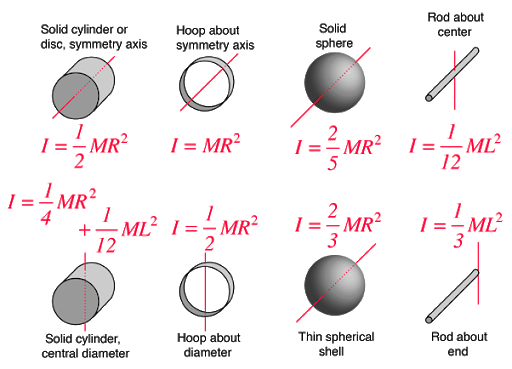
\includegraphics[width=0.4\textwidth]{moment-of-inertia.png}
\end{center}

\section{Angular Momentum}
\subsection{Centre of Mass}
\begin{align*}
    V_{cm} &= R \omega \\
    a_{cm} &= R \alpha \\
    d_{cm} &= R \theta \\
    L &= I \omega \\
    L &= mvr \quad \textrm{(for point object)} \\
    \Delta L &= \tau \Delta t \\
    T &= \frac{2 \pi}{\omega} = \frac{1}{f}
\end{align*}

\medskip
\begin{center}
    \textbf{ANGULAR MOMENTUM MUST BE CONSERVED}
\end{center}

\appendix
\section*{Terms/Definitions}

\section*{Constants}

\section*{Conversions}

\section*{Orders of Magnitude}

\section*{Trigonometry}

\section*{Calculus}

\end{multicols}
\end{document}

